\section{BROADR}
\label{sBROADR}

\hypertarget{sBROADRhy}{BROADR}
\index{BROADR|textbf} module generates
Doppler-broadened\index{Doppler-broadening}
cross sections in PENDF\index{PENDF} format starting from piecewise
linear cross sections in PENDF format.  The input cross sections can
be from \hyperlink{sRECONRhy}{RECONR}\index{RECONR} or
from a previous BROADR run.  The code is
based on SIGMA1\cite{SIGMA1}\index{SIGMA1} by D. E. Cullen.\index{Cullen}
The method is often called ``kernel broadening''\index{kernel broadening}
because it uses a detailed integration of the integral equation defining
the effective cross section.  It is a fully accurate method,
treating all resonance and non-resonance cross sections including
multilevel effects.  BROADR has the following features:
\begin{itemize}
\begin{singlespace}
\item An alternate calculation is used for low energies
      and high temperatures that corrects a numerical problem of
      the original SIGMA1. (This problem has been corrected
      in another way in later versions of SIGMA1.)

\item Dynamic storage allocation is used, which allows the code
      to be run on large or small machines with full use of whatever
      storage is made available.

\item Reactions are broadened in parallel on a union grid, with the top
      of the resolved resonance range being the typical upper limit
      for Doppler broadening.

\item The union grid is constructed adaptively to give
      a linearized representation of the broadened cross section
      with tolerances consistent with those used in
      \hyperlink{sRECONRhy}{RECONR}.  Energy
      points may be added to or removed from the
      input grid as required for the best possible
      representation.  Precision up to 9 significant figures
      is allowed for energies.

\item The summation cross sections such as total, nonelastic, and
      sometimes fission or (n,2n) are reconstructed to equal the
      sum of their parts.

\item Standard thermal cross sections, integrals, and ratios are
      computed when the temperature is 293.6K (0.0253 eV).

\item The file directory (actually an index to the
      reactions present) is updated.
\end{singlespace}
\end{itemize}

This chapter describes the BROADR module in NJOY2016.0.

\subsection{Doppler-Broadening Theory}
\label{ssBROADR_theory}

The effective cross section for a material at temperature $T$ is
defined to be that cross section that gives the same reaction rate
for stationary target nuclei as the real cross section gives for
moving nuclei.  Therefore,
\begin{equation}
  \rho v {\overline \sigma}(v,T)=
    \int d{\bf v}' \rho\,|{\bf v}-{\bf v}'|\,\sigma(|{\bf v}-{\bf v}'|
    )\,P({\bf v}',T)\,\,,
\label{effxs}
\end{equation}
where ${\bf v}$ is the velocity of the incident particles,
${\bf v}'$ is the velocity of the target, $\rho$ is the density
of target nuclei, $\sigma$ is the cross section for stationary
nuclei, and $P({\bf v}',T)$ is the distribution of target
velocities in the laboratory system.  For many cases of interest,
the target motion is isotropic and the distribution of velocities
can be described by the Maxwell-Boltzmann\index{Maxwell-Boltzmann function}
function
\begin{equation}
  P({\bf v}',T)\,d{\bf v}'=
    {{\alpha^{3/2}} \over {\pi^{3/2}}} \exp (-\alpha {v'}^2)\,
    d{\bf v}'\,\,,
\end{equation}
where $\alpha=M/(2kT)$, $k$ is Boltzmann's constant\index{Boltzmann
constant}, and $M$ is the target mass.

Eq.~\ref{effxs} can be partially integrated in terms of the
relative speed $V=|{\bf v}-{\bf v}'|$ to give the standard form
of the Doppler-broadened cross section:
\begin{equation}
  {\overline\sigma}(v)={{\alpha^{1/2}} \over {\phi^{1/2}\,v^2}}
    \int_0^\infty dV\,\sigma(V)\,V^2\,\Bigl\lbrace
    {\rm e}^{-\alpha (V-v)^2}-{\rm e}^{-\alpha (V+v)^2}
    \Bigr\rbrace \,\,.
\label{standform}
\end{equation}
It is instructive to break this up into two parts:
\begin{equation}
  {\overline\sigma}(v)=\sigma^* (v)-\sigma^*(-v)\,\,,
\end{equation}
where
\begin{equation}
  \sigma^*(v)={{\alpha^{1/2}} \over {\pi^{1/2}v^2}}
    \int_0^\infty dV\,\sigma(V)\,V^2\,{\rm e}
    ^{-\alpha (V-v)^2} \,\,.
\label{sigv}
\end{equation}

\noindent
The exponential function in Eq.~(\ref{sigv}) limits the
significant part of the integral to the range
\begin{displaymath}
  v-{{4}\over {\sqrt{\alpha}}} < V
    <v+{{4} \over {\sqrt{\alpha}}} .
\end{displaymath}
For $\sigma^*(-v)$, the integral depends only on velocities
satisfying
\begin{displaymath}
   0\le V<{{4}\over{\sqrt{\alpha}}} .
\end{displaymath}
These results can be converted to energy units using
\begin{displaymath}
E_m={1\over 2} m \bigl( {4 \over \sqrt{\alpha}} \bigr)^2
    = {{16kT} \over A}.
\end{displaymath}
Some examples are given in Table~\ref{T1}.  Doppler-broadening effects
will be important below this energy and for any features such as
resonances, thresholds, or artificial discontinuities in
evaluations that are not slowly varying with respect to
$2\sqrt{E_mE}$.  As an example, for $^{235}$U at 100 eV, Doppler
effects are important for features smaller than about 0.8 eV.

\begin{table}
\caption[Energy Parameter for Effective Doppler-Broadening]
 {Energy Parameter for Effective Doppler-Broadening}
\setlength{\extrarowheight}{1pt}
\label{T1}
\begin{center}
\begin{tabular}{lcc}
Target & Temperature & Energy Parameter ($E_m$) \\
\hline
$^{2}$H & 300K & 0.2 eV \\
$^{235}$U & 300K & 0.0017 eV \\
$^{235}$U & 1.0 keV & 69 eV \\
\hline
\end{tabular}
\end{center}
\end{table}

The numerical evaluation of Eq.~(\ref{sigv}) developed for SIGMA1
assumes that the cross section can be represented by a piecewise
linear function of energy to acceptable accuracy.  This is just
the form of the NJOY PENDF\index{PENDF} files (see
\hyperlink{sRECONRhy}{RECONR}\index{RECONR}).  Defining the
reduced variables $y=\sqrt{\alpha x}$ and $x=\sqrt{\alpha V}$,
the cross section becomes
\begin{equation}
  \sigma (x)=\sigma_i + s_i (x^2-x_i^2 )\,\,,
\label{sigmax}
\end{equation}
with slope $s_i=(\sigma_{i+1}-\sigma_i)/(x_{i+1}^2-x_i^2 )$.
Eq.~(\ref{sigv}) can now be written as
\begin{equation}
  \sigma^*(y)={{1} \over{\pi^{1/2}y^2}}
    \sum_{i=0}^N \int_{x_i}^{x_{i+1}}
    \sigma (x)\,x^2 {\rm e}^{-(x-y)^2}dx
    = \sum_i \bigl\lbrace A_i\,[\sigma_i-s_i x_i^2]+
    B_i s_i \bigr\rbrace \,\,,
\label{sigy}
\end{equation}
where
\begin{eqnarray}
  x_0&=&0\,\,,\nonumber\\
  x_{N+1}&=&\infty\,\,,\nonumber\\
  A_i&=&{1\over y^2}H_2+{2\over y}H_1+H_0\,\,,\;\hbox{and}\nonumber\\
  B_i&=&{1\over y^2}H_4+{4\over y}H_3+6H_2+4yH_1+y^2 H_0\nonumber \,\,,
\end{eqnarray}
and where $H_n$ is shorthand for $H_n(x_i{-}y,x_{i+1}{-}y)$.  The
extrapolations to zero and infinity assume a constant cross section
($s_0{=}s_N{=}0$).  The $H$ functions are the incomplete
probability integrals\index{incomplete probability integral}
\index{math!incomplete probability integral} defined by
\begin{equation}
  H_n(a,b)={1\over \sqrt{\pi}} \int_a^b
    z^n\,{\rm e}^{-z^2}\,dz\,\,.
\label{fn}
\end{equation}
These functions can be computed in two ways.  First,
\begin{equation}
  H_n(a,b)=F_n(a)-F_n(b)\,\,,
\label{diffs}
\end{equation}
where
\begin{equation}
  F_n(a)={1\over \sqrt{\pi}}\int_a^\infty z^n\,{\rm e}^{-z^2}\,dz\,\,.
\end{equation}
These functions satisfy a recursion relation that can be used
to obtain
\begin{eqnarray}
  F_0(a)&=&{1\over 2} {\rm erfc}(a)\,\,,\\
  F_1(a)&=&{1\over {2\sqrt{\pi}}} \exp(-a^2)\,\,,\;\hbox{and}\\
  F_n(a)&=&{{n-1} \over 2}F_{n-2}(a)+a^{n-1}F_1(a)\,\,,
\label{recur}
\end{eqnarray}
where ${\rm erfc}(a)$ denotes the complementary error function
\index{complementary error function}
\index{math!complementary error function}
\begin{equation}
  {\rm erfc}(a)={2\over \sqrt{\pi}}
    \int_a^\infty {\rm e}^{-z^2}dz\,\,.
\end{equation}
However, when $F_n(a)\approx F_n(b)$, the difference in
Eq.~(\ref{diffs}) may lose significance.  In such cases,
$H_n(a,b)$ can be computed by a second method based on a
direct Taylor expansion of the defining integral.  Write
\begin{equation}
  H_n(a,b)={1\over \sqrt{\pi}}\int_0^b z^n {\rm e}^{-z}
    dz-{1\over \sqrt{\pi}}\int_0^a z^n {\rm e}^{-z^2}dz
    =G_n(b)-G_n(a)\,\,.
\label{alt1}
\end{equation}
But by Taylor's Theorem,
\begin{equation}
  G_n(b)-G_n(a)=
    {{b-a}\over {1!}}G'_n(a)+...+
    {{(b-a)^m}\over{m!}}G_n^{(m)}(a)+... \,.
\end{equation}
Also,
\begin{equation}
  G_n^{(m)}(x)={{d^{m-1}}\over{dx^{m-1}}}
    \bigl[ x^n{\rm e}^{-x^2} \bigr] =
    {\rm e}^{-x^2} P_n^m(x)\,,
\end{equation}
where $P_n^m(x)$ is a polynomial with recursion relation
\begin{equation}
  P_n^m(x)={d\over{dx}}P_n^{m-1}(x)-2xP_n^{m-1}(x)\,\,,
\label{alt2}
\end{equation}
with $P_n^1=x^n$.  From this point, it is straightforward to
generate terms until the desired number of significant figures
is obtained.

\begin{figure}[t]\centering
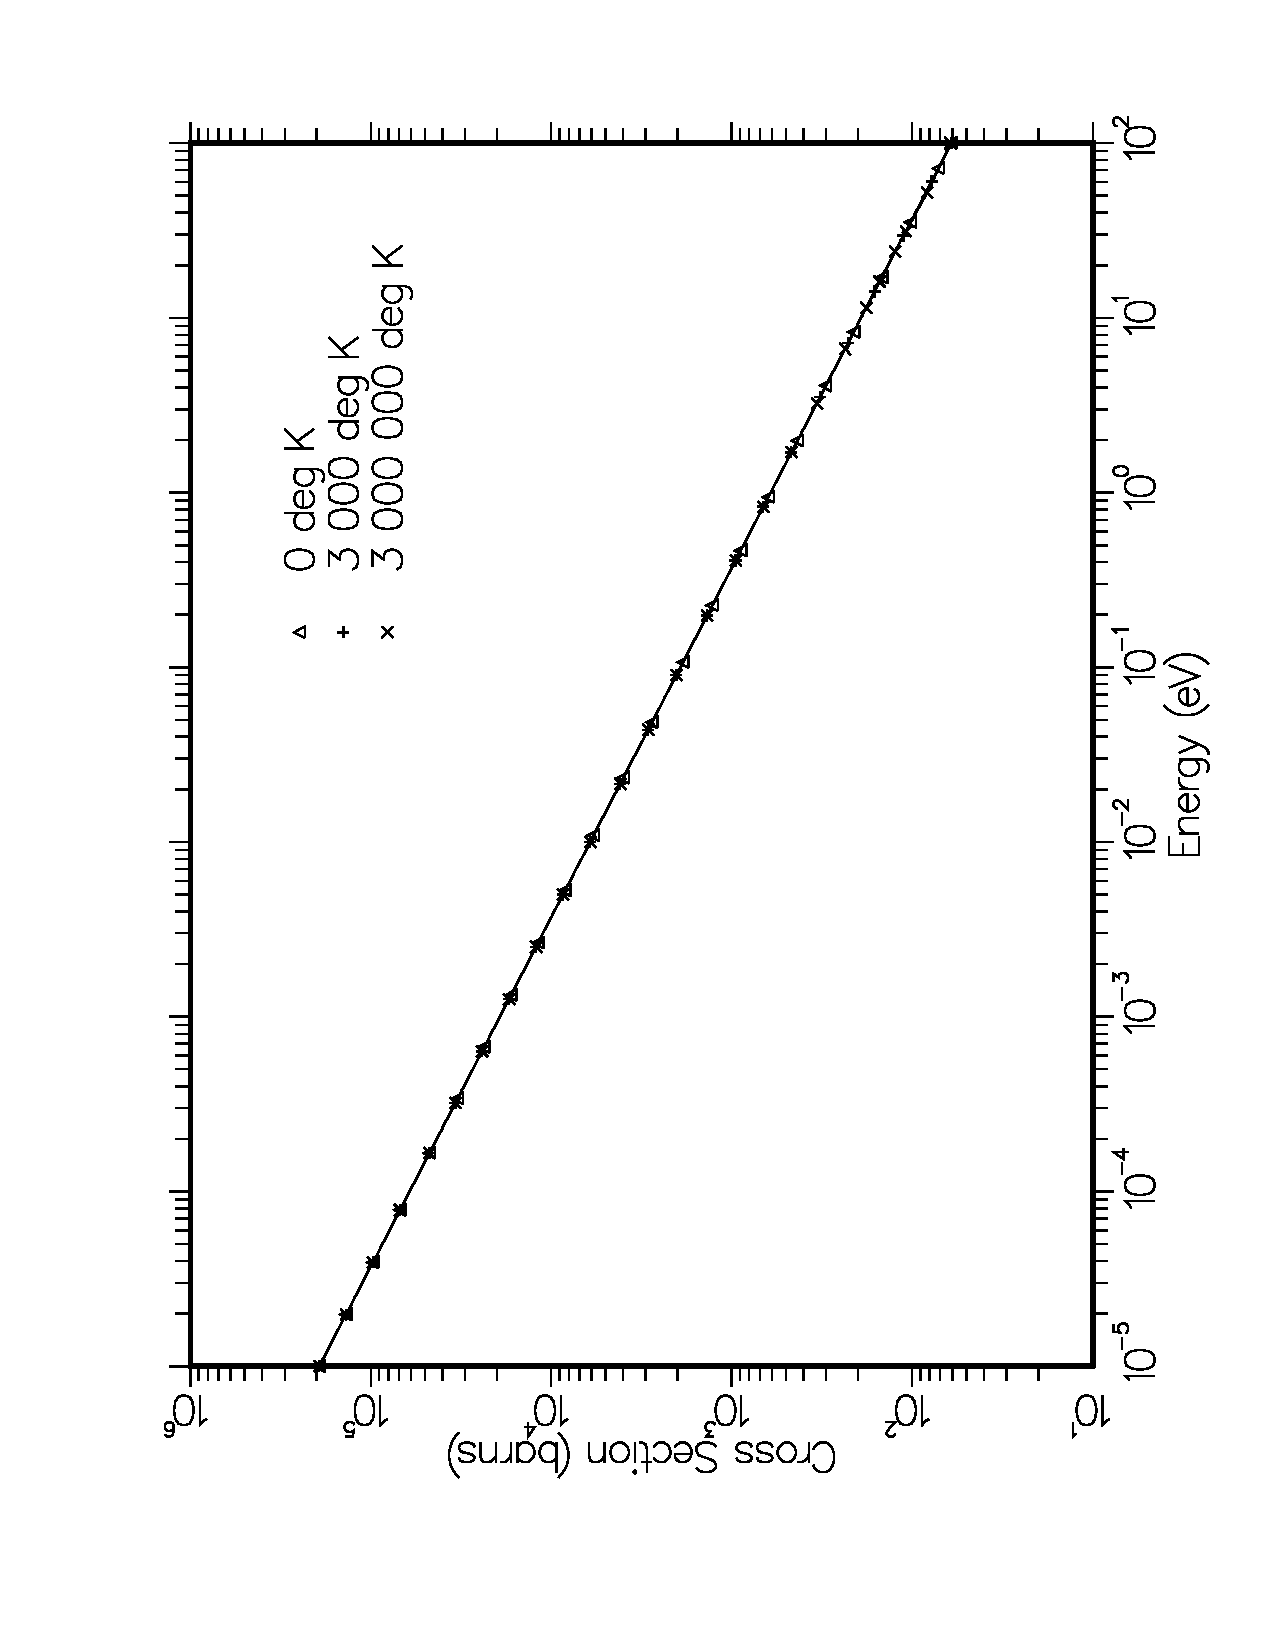
\includegraphics[keepaspectratio, height=4.0in, angle=270]{figs/broadr1ack}
\caption[The $^{10}$B (n,$\alpha$) cross section versus Doppler broadening
temperature]
{The (n,$\alpha$) cross section for $^{10}$B
        from ENDF/B-V for three different temperatures showing that
        a $1/v$ cross section is invariant under Doppler-broadening.}
\label{over}
\end{figure}

When interpreting BROADR output, it is useful to remember several
important features of the Doppler-broadening process.
\index{Doppler-broadening}
A $1/v$ cross section remains unchanged.  Contrary to ``popular
knowledge'', the area under a resonance does not remain unchanged
unless $E\gg kT/A$.  In fact, each resonance develops a new $1/v$
tail.  Finally, a constant cross section (for example, elastic
scattering) develops a $1/v$ tail at low energies after
Doppler-broadening.  These effects are shown in Figs.~\ref{over},
\ref{elas}, and \ref{reson};  they can be best understood by noting
that the Doppler process preserves reaction rate $v\sigma (v)$
according to Eq.~(\ref{effxs}), and a finite reaction rate is
expected for $T>0$K even as $v\rightarrow 0$.

\begin{figure}[thbp]\centering
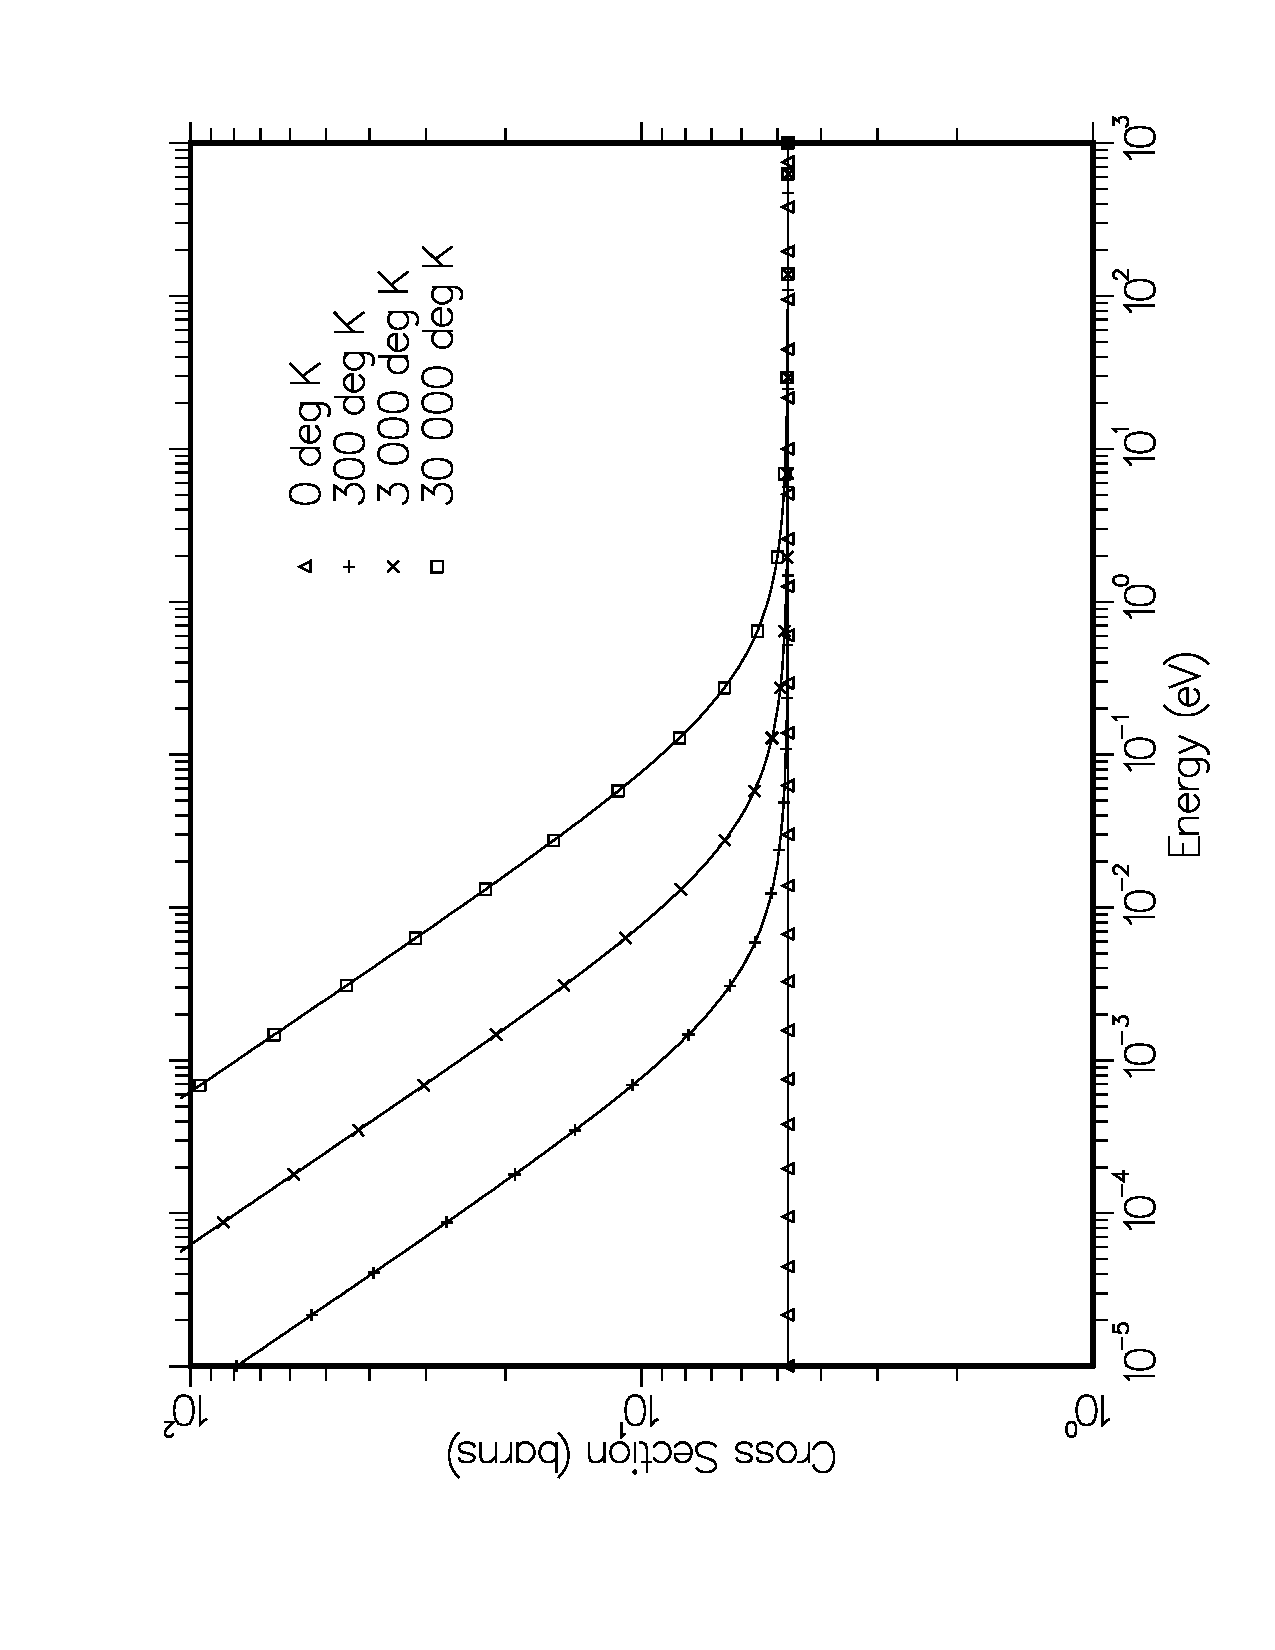
\includegraphics[height=4.0in, angle=270]{figs/broadr2ack}
\caption[The $^{nat}$C elastic scattering cross section versus Doppler
 broadening temperature]
{The elastic cross section for carbon
        from ENDF/B-V showing that Doppler-broadening a constant
        cross section adds a $1/v$ tail.}
\label{elas}
\end{figure}

\begin{figure}[thbp]\centering
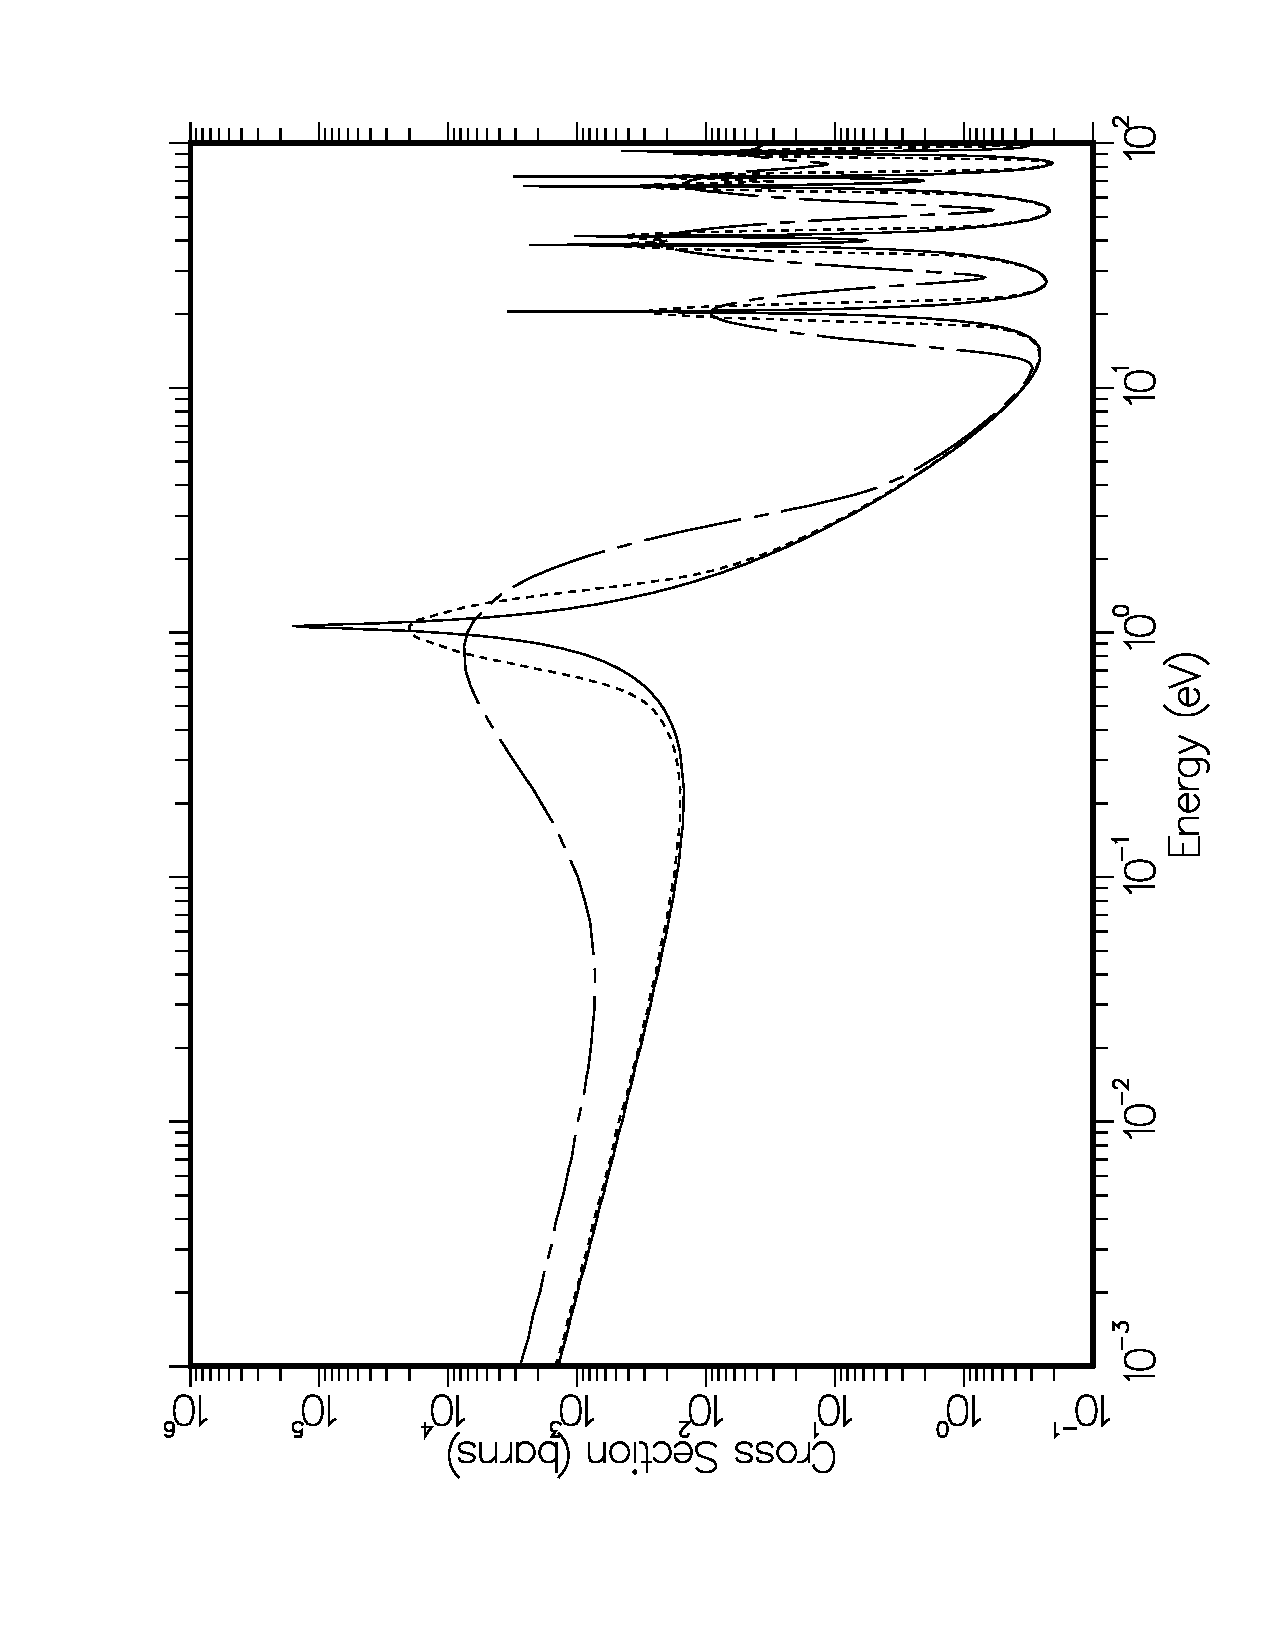
\includegraphics[keepaspectratio, height=3.6in, angle=270]{figs/broadr3ack}
\caption[The $^{240}$Pu low energy (n,$\gamma$) cross section versus Doppler
 broadening temperature]
{The (n,$\gamma$) cross section for
 $^{240}$Pu for several temperatures showing
 the effects of Doppler broadening on resonances.  The
 temperatures are 0K (solid), 30\ 000K (dotted), and
 300\ 000K (dash-dot).  The higher resonances behave in
 the classical manner even at 30\ 000K; note that the
 line shape returns to the asymptotic value in the wings
 of the resonance.  All resonances at 300\ 000K (and to a
 lesser extent the first resonance for 30\ 000K) show the
 additional $1/v$ component that appears when $kT/A$ is
 large with respect to the resonance energy.}
   \label{reson}
\end{figure}

Very early (1980s) versions of BROADR and SIGMA1 assumed that the input
energy grid from \hyperlink{sRECONRhy}{RECONR}\index{RECONR}
could also be used to represent
the Doppler-broadened cross section before thinning.  The grid was
then thinned to take advantage of the smoothing effect of Doppler
broadening.  Unfortunately, this assumption is inadequate.  The
reconstruction process in \hyperlink{sRECONRhy}{RECONR} places many points
near the center of a resonance to represent its sharp sides.  After
broadening, the cross section in this energy region becomes
rather smooth;  the sharp sides are moved out to energies where
\hyperlink{sRECONRhy}{RECONR} provides few points.  At still higher energies,
the resonance line shape returns to its asymptotic value, and the
\hyperlink{sRECONRhy}{RECONR} grid is adequate once more.  The more recent
versions of BROADR check the cross section between points of the incoming
energy grid, and add additional grid points if they are necessary
to represent the broadened line shape to the desired accuracy.
This effect is illustrated in Fig.~\ref{grids}.

\begin{figure}[t]\centering
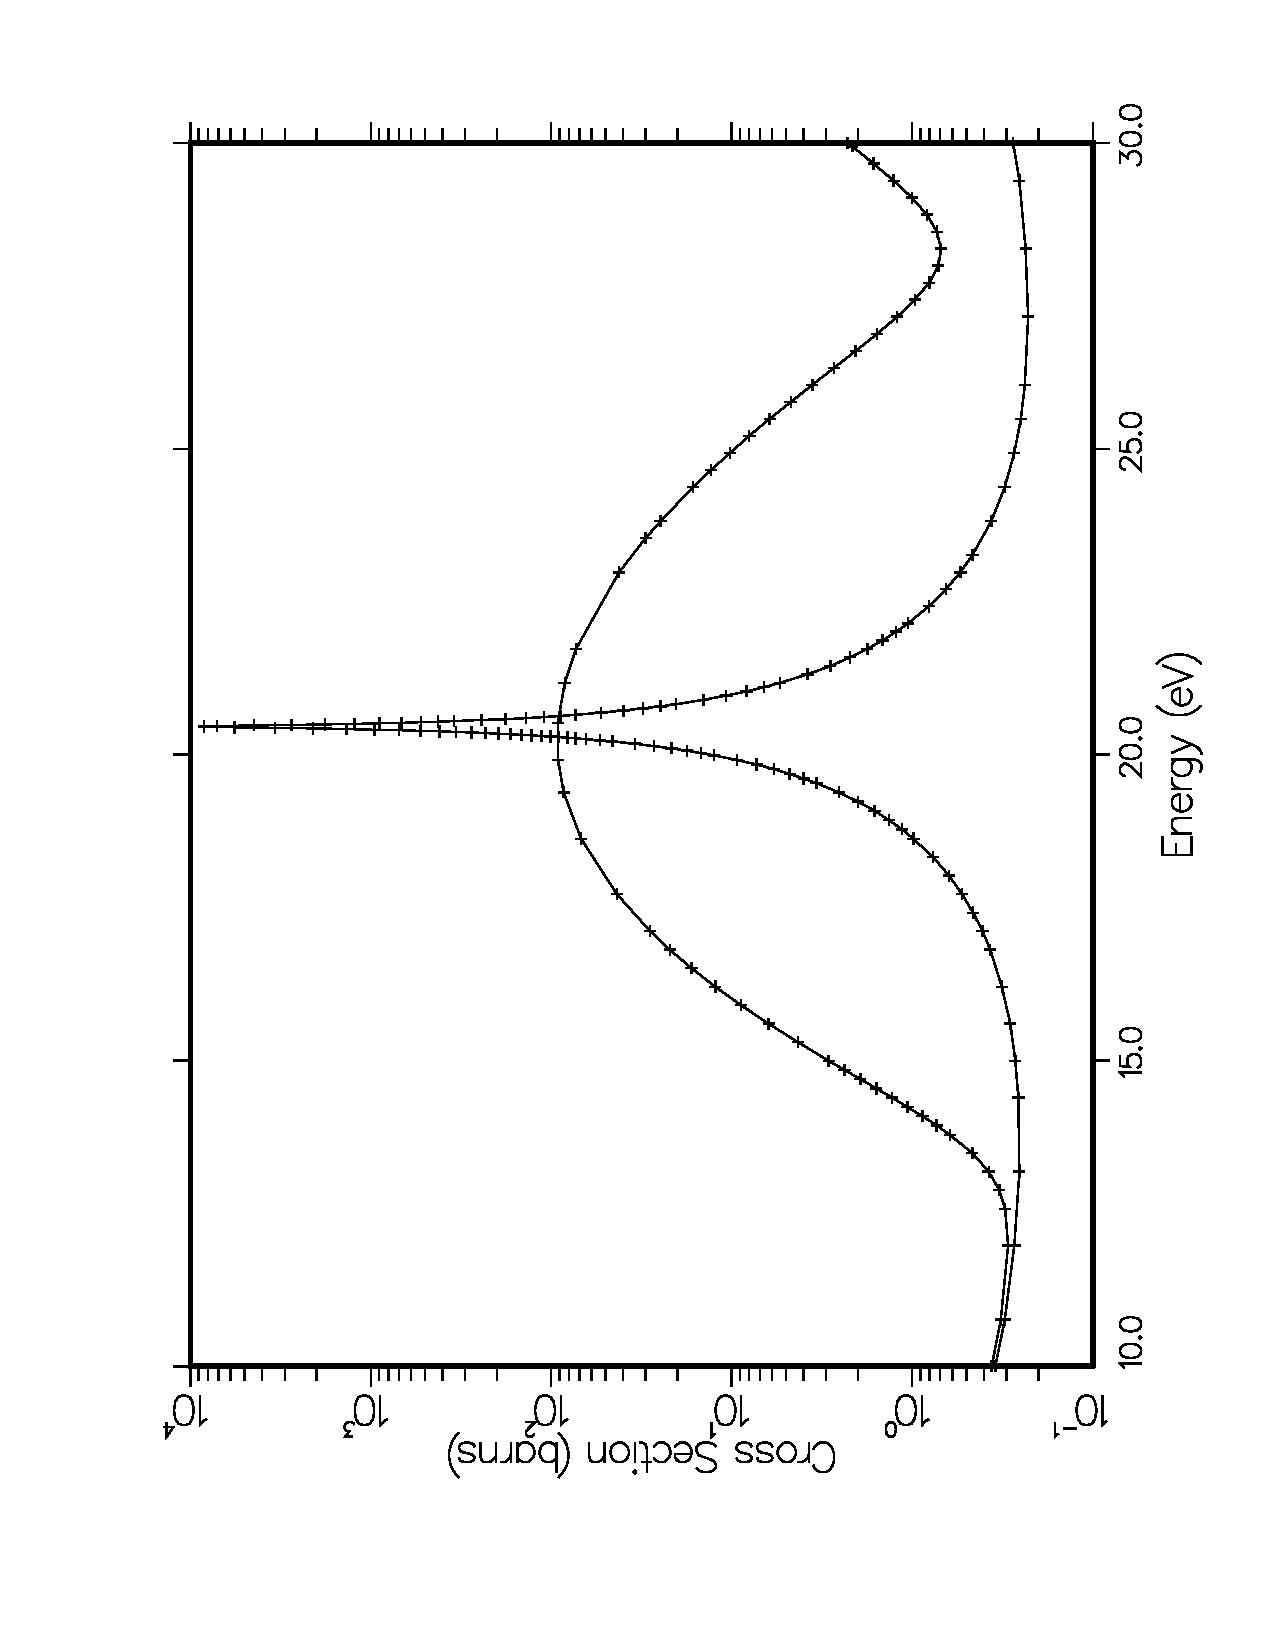
\includegraphics[keepaspectratio, height=3.6in, angle=270]{figs/broadr4ack}
\caption[Energy grid variation with Doppler broadening]{An expanded plot
 of the 20 eV resonance  from Fig.~\ref{reson} showing both thinning
 and ``thickening'' of the energy grid produced adaptively
 by BROADR.  The two curves show the capture cross section
 at 0K and 300 000K.  Note that the high-temperature
 curve has fewer points than the 0K curve near the peak
 at 20 eV and more  points in the wings near 15 eV and 25
 eV.  Clearly, using the 0K grid to represent the
 broadened cross section in the wings of this resonance
 would give poor results.}
   \label{grids}
\end{figure}

\subsection{Thermal Quantities}
\label{ssBROADR_thermal}

In thermal-reactor work, people make very effective use of a few
standard thermal constants\index{thermal constants} to
characterize nuclear systems.  These parameters include
the cross sections at the standard thermal value of
0.0253 eV (2200 m/s), the integrals of the cross sections
against a Maxwellian distribution for 0.0253 eV, the g-factors
(which express the ratio between a Maxwellian integral and the
corresponding thermal cross section), $\eta$, $\alpha$, and K1.
Here, $\eta$ is the Maxwellian-weighted average of
$(\bar{\nu)}\sigma_f)/(\sigma_f+\sigma_c)$, $\alpha$ is
the average of $\sigma_c/\sigma_f$, and K1 is the average
of $(\bar{\nu}-1)\sigma_f-\sigma_c$.  If BROADR is run for a
temperature close to 293.6K (which is equivalent to 0.0253 eV),
these thermal quantities are automatically calculated and displayed.
Here is a sample output for $^{235}$U from ENDF/B-VII\index{ENDF!ENDF/B-VII}:

\small
\begin{ccode}

    thermal quantities at 293.6 K = 0.0253 eV
    -----------------------------------------
           thermal fission xsec:  5.8490E+02
          thermal fission nubar:  2.4367E+00
           thermal capture xsec:  9.8665E+01
       thermal capture g-factor:  9.9086E-01
       thermal capture integral:  8.6639E+01
     capture resonance integral:  1.4043E+02
       thermal fission integral:  5.0605E+02
       thermal fission g-factor:  9.7628E-01
         thermal alpha integral:  1.6828E-01
           thermal eta integral:  2.0859E+00
            thermal k1 integral:  6.4040E+02
                  equivalent k1:  7.2262E+02
     fission resonance integral:  2.7596E+02
    -----------------------------------------

\end{ccode}
\normalsize

\subsection{Data-Paging Methodology}
\label{ssBROADR_paging}

A piecewise linear representation of a reaction cross section of
a resonance material may require a very large number of energy
points.  For example, ENDF/B-VII $^{238}$U (MAT9237) requires 167\ 000
points for the total cross section for 0.1\% precision
(\cword{errmax}=\cword{err}).  It is impractical to load all these points
into memory simultaneously.  However, the discussion following
Eq.~(\ref{sigv}) in the theory section shows that only a limited
energy range around the point of interest is required.

The strategy used is to stage the cross-section data into three
``pages'' of \cword{npage} points each.\index{paging}  Points in
the center page can then be broadened using the \cword{npage} or
more points on each side of the point of interest.  If
$v-4/\sqrt{\alpha}$ and $v+4/\sqrt{\alpha}$ are both included in
the three-page range, accurate broadening can be performed.  If
not, a diagnostic warning is printed; the user should repeat the
calculation with a smaller temperature step or a larger page
size.

There are many different reaction cross sections for each
material.  However, the cross sections for high velocities are
normally smooth with respect to $32kT/A$ for any temperatures
outside of stellar photospheres; therefore, they do not show
significant Doppler effects.  Until recently the upper energy limit
for Doppler broadening was the smallest of (i) the input value
\cword{thnmax}, (ii) the upper limit of the resolved-resonance
energy range, (iii) the lowest threshold, or (iv) 1.0 MeV
(the default input value for \cword{thnmax}).  No Doppler
broadening or energy-grid reconstruction is performed
above that energy.  In the past, and what users
typically expect as the default action, the second condition
often set the Doppler broadening upper limit.

However recent evaluated files have increasingly included threshold
reactions at energies within the resolved resonance energy
range.  For example, recent JENDL evaluations for $^{235}$U include a
resolved-resonance range upper limit of 2.25 keV, but also
include non-zero cross sections for an inelastic level with a 77 eV
threshold.  Under the rules itemized above, Doppler broadening of
these data stops at 77 eV.  Other evaluations ({\it e.g.}, ENDF/B-VI,
ENDF/B-VII and JEFF-3.1) share the same resolved-resonance range data but
have zeroed out this inelastic cross section from 77 eV to 2.25 keV
and so Doppler broadening of these files occurs throughout the
resolved-resonance range, as most users expect.

Zeroing out non-zero data is a cludge from the past and so we have
changed the Doppler upper energy limit logic so that the top of the
resolved resonance range is now the default condition.  This means
that non-threshold reactions are also Doppler broadened.  The
mathematics of this operation can produce non-zero cross sections
at energies below the reaction threshold.  If this occurs those
cross sections are zeroed.

As noted in the BROADR module source code comments, users
may specify a negative value for \cword{thnmax} to override these
selection rules and force Doppler broadening to an upper energy
of \cword{abs(thnmax)} eV.  This has been a long-term NJOY feature
that remains unchanged in NJOY2016.

Finally, we note that the $A_i$ and $B_i$
factors in Eq.~(\ref{sigy}) depend only on the energy (or
velocity) values and not on the cross sections.  Since the $A_i$
and $B_i$ are expensive to compute, the code computes them only
once for the points of a unionized energy grid.  The sum of
Eq.~(\ref{sigy}) is accumulated for all the non-threshold
reactions simultaneously.  This feature helps make BROADR run
faster.

\subsection{Coding Details}
\label{ssBROADR_details}

The main subroutine for BROADR is
\cword{broadr}\index{broadr@{\ty broadr}} from
module \cword{broadm}\index{modules!broadm@{\ty broadm}}.  The
code begins by reading the user's input (see Section~\ref{ssBROADR_inp}).
Storage is then allocated for the \cword{loada/finda} buffers
(\cword{ibufo} and \cword{ibufn}) and for the scratch storage
(\cword{iscr}).  The buffer length \cword{nbuf} can be changed at
will (currently \cword{nbuf} is 1000).

The input PENDF\index{PENDF} tape is searched for the desired material
(\cword{mat1}).  If the restart option is set (\cword{istart}=1),
the temperatures less than or equal to \cword{temp1} for
\cword{mat1} are assumed to have been broadened previously, and
they are copied to the output file.  In either case, the files
for \cword{temp1} are copied to a scratch file on unit
\cword{nscr1}.

Next, \cword{nscr1} is rewound and examined reaction by
reaction.  The energy grid from the total cross section (MT1) is
saved on scratch storage using \cword{loada}.  If the input tape
has not been through \hyperlink{sRECONRhy}{RECONR}\index{RECONR},
the BROADR module will
still run, but at possibly reduced accuracy.  The next low-threshold
reaction (that is, the next reaction with a threshold less than
\cword{emin}, which is currently 1 eV) is located on
\cword{nscr1}.  The energy points are retrieved from scratch file
\cword{iold} (12 or 13) using \cword{finda}, the cross sections
for this reaction are computed on this grid, and the results are
stored on scratch file \cword{inew} (13 or 12) using
\cword{loada}.  The units for \cword{iold} and \cword{inew} are
then exchanged, and the entire process is repeated for the next
low-threshold reaction.

The final result of this process is a list of \cword{nreac}
low-threshold-reaction types in \cword{mtr} (usually MT2, MT18,
and MT102), the threshold value for the first high-threshold
reaction (or the input value) in \cword{thnmax}, and scratch file
\cword{iold} containing the energy grid and all the low-threshold
reactions (there are \cword{n2in} points).

Now that the number of reactions to be broadened simultaneously
is known (\cword{nreac}), storage for data paging can be assigned.
The total amount of storage available is \cword{namax}.  The value
of \cword{namax} should be as large as possible (current value
is 15\ 000\ 000).  This space is divided up into the largest possible
page size, \cword{npage}.  An overflow region \cword{nstack} is also
allocated.  Now that the page size is known, the code allocates three
pages for energies (\cword{e}), three pages for each reaction
cross section (\cword{s}), one extended page for the broadened
energy grid (\cword{eb}), and three extended pages for the
broadened cross section (\cword{sb}).  This system is designed to
use the available storage with maximum efficiency.

The cross sections on \cword{iold} are now broadened by
\cword{bfile3}\index{bfile3@{\ty bfile3}} (see below) and the results
are written on scratch unit \cword{inew} using \cword{loada}.

The directory from \cword{nscr1} is revised to reflect any thinning
or thickening and written on the output PENDF tape (\cword{nout}).
Note that the new temperature is written into the first word of the
Hollerith data record to simplify later searching.

The broadened cross sections are now converted into ENDF TAB1
\index{TAB1@{\ty TAB1}} records and merged with the unbroadened
cross sections on \cword{nscr1}.  The total cross section (and
sometimes nonelastic, inelastic, fission, (n,2n), or
charged-particle reactions) is reconstructed to equal the
sum of its parts\index{summation cross sections}.  The new
Doppler-broadened ``MAT'' on \cword{NOUT} is a legal PENDF file
with the same MAT number as the original data but with a
new temperature.

The process is now repeated for each of the \cword{ntemp2} final
temperatures \cword{temp2} requested.  Note that after each step
\cword{inew} contains the new data and \cword{iold} contains the
previous data.  If the ``bootstrap'' option is set
(\cword{istrap}=1), these units are interchanged.  For this
option, \cword{stemp2(it)} is always obtained from
\cword{temp2(it-1)}.  Because of the thinning effect of
Doppler-broadening, the broadening runs faster at each step.  The
accumulation of error is usually not a problem.  For
\cword{istrap}=0, \cword{temp1} is used for the starting
temperature every time.

The broadening and energy-grid reconstruction are directed by
\cword{bfile3}\index{bfile3@{\ty bfile3}} .  The routine loads data
into the appropriate memory pages from scratch file \cword{iold} and
then either calls \cword{broadn}\index{broadn@{\ty broadn}}
to broaden it (with thinning or thickening of the grid as necessary)
or calls \cword{thinb}\index{thinb@{\ty thinb}} to thin
it without broadening.  The results are written onto scratch file
\cword{inew}.

In \cword{broadn}\index{broadn@{\ty broadn}}, the energy grid points
just loaded into \cword{e} by \cword{bfile3}\index{bfile3@{\ty bfile3}}
are converted to the dimensionless variables x and y
[see Eq.~(\ref{sigmax})].  An adaptive reconstruction
\index{adaptive reconstruction} of the Doppler broadened
cross section is then performed for the energy range in the
center page using an inverted stack\index{inverted stack}
algorithm like the one described for
\hyperlink{sRECONRhy}{RECONR}\index{RECONR}.  The
upper limit of each panel is taken to be a point from the input
grid, but in order to allow for thinning, up to \cword{nmax}=10
of the input grid points can be skipped before the actual upper
limit is selected.  In addition, the energy of the upper limit
cannot be more than \cword{step}=2.01 times the energy of the
preceding point.  The cross sections are now computed at the
midpoint of the top panel in the stack using \cword{bsigma}.  If
the results differ from the values obtained by interpolation by
more than the specified tolerance, the new point is added to the
stack, and the tests are repeated.  Otherwise, the top point in
the stack is converged.  A backward check is made to see if some
of the previous points can be removed based on the new value, the
new value is stored in the output array, and the height of the
stack is reduced by one.   The routine now tries to subdivide the
new panel at the top of the stack in the same way.  When the
stack has been reduced to one element, a new upper limit is
chosen from the input energy grid as described above, and the
entire process is repeated.  The reconstruction logic in BROADR
uses the same integral tests as
\hyperlink{sRECONRhy}{RECONR}\index{RECONR}.  Refer to
the \hyperlink{sRECONRhy}{RECONR} chapter for more details.

Subroutine \cword{bsigma}\index{bsigma@{\ty bsigma}} is used
to calculate the actual broadened cross section at an energy
point using the data in the three pages.  First, the routine
locates the energy panel containing the desired energy \cword{en}.
It then loops over intervals below the current point adding in
contributions to $\bar{\sigma}$ from the $V{-}v$ term of
Eq.~(\ref{standform}) until the contributions to the cross section
become small.  If the lower limit of the bottom page is reached
before convergence, a warning message is issued.  The routine
then loops over intervals above the current point until
convergence.  Once again, a warning is issued if necessary.
Finally, the low-energy term [the one involving
$V{+}v$ in Eq.~(\ref{standform})] is added, if applicable.

Subroutine \cword{thinb}\index{thinb@{\ty thinb}} is provided
for cases where the input cross section set is to be thinned only.
 This routine uses the original SIGMA1\index{SIGMA1} method.  The
first input point is always kept.  The routine then loops over
higher energy values.  For each grid point, all the points from
there back to the last accepted point are checked for their
deviation from a straight line.  If they all can be removed
without violating the specified tolerance, the interval is
extended to the next higher point and the tests are
repeated.  If any point in the range is too far from the linear
approximation, the last point in the range is accepted as an
output point, and the testing process is repeated starting from
this new lower limit.  The procedure terminates when all of the
points in the middle page have been thinned, and control is
returned to \cword{bfile3}\index{bfile3@{\ty bfile3}} to get
the next page of data.  Thinning may have been a necessary
feature in the past when computing resources were limited but
is a rarely used feature today.

Subroutine \cword{hunky}\index{hunky@{\ty hunky}} has been modified
from the original SIGMA1 version to implement the alternate
$H_n(a,b)$ calculation when necessary (see
\cword{hnabb}\index{hnabb@{\ty hnabb}}).  When using the direct
method, $F_n$ values from the previous step are used in the
difference of Eq.~(\ref{diffs}), and \cword{funky} is called to
get the new values.  The $A_i$ and $B_i$ of Eq.~(\ref{sigy}) are
related to the \cword{s1} and \cword{s2} here.

Subroutine \cword{funky}\index{funky@{\ty funky}} evaluates
$F_n(a)$ by the recursion formula of Eq.~(\ref{recur}) using
the very accurate SLATEC\index{SLATEC} version of
the reduced complementary error function
\index{complementary error function} from the NJOY2016
math module\index{modules!math@{\ty math}}.

Function \cword{hnabb}\index{hnabb@{\ty hnabb}} implements the
alternate calculation described by Eqs.~(\ref{alt1})-(\ref{alt2}).
The series expansion is continued until about six significant figures
are guaranteed (see \cword{eps} and \cword{hnabb}).  Currently,
\cword{hnabb} is called when only four significant figures are
reliable in \cword{hunky} (see \cword{toler} in \cword{hunky}).

\subsection{User Input}
\label{ssBROADR_inp}

The following input instructions have been copied from the
comment cards at the start of BROADR.
\index{BROADR!BROADR input}
\index{input!BROADR}

\small
\begin{ccode}

   !---input specifications (free format)---------------------------
   !
   ! card 1
   !    nendf    input endf tape (for thermal nubar only)
   !    nin      input pendf tape
   !    nout     output pendf tape
   !
   ! card 2
   !    mat1     material to broadened and thinned
   !    ntemp2   number of final temperatures (default=1)
   !    istart   restart (0 no, 1 yes, default 0)
   !    istrap   bootstrap (0 no, 1 yes, default 0
   !    temp1    starting temperature from nin (default=0K)
   !
   ! card 3
   !    errthn   fractional tolerance for thinning
   !    thnmax   max. energy for broadening and thinning
   !             (default=1 MeV)
   !    errmax   fractional tolerance used when integral criterion
   !             is satisfied (same usage as in reconr)
   !             (errmax.ge.errthn, default=10*errthn)
   !    errint   parameter to control integral thinning
   !             (usage as in reconr) (default=errthn/20000)
   !             set very small to turn off integral thinning.
   !      (A good choice for the convergence parameters
   !       errthn, errmax, and errint is the same set of
   !       values used in reconr)
   !
   ! card 4
   !    temp2    final temperatures (deg Kelvin)
   !
   ! card 5
   !    mat1     next MAT number to be processed with these
   !             parameters.  Terminate with mat1=0.
   !
   !---input options------------------------------------------------
   !
   ! The output tape will contain the ntemp2 final temperatures
   ! specified.  It is necessary to have temp1.le.temp2(1).
   ! if temp2.eq.temp1, the data will be thinned only.
   !
   ! restart    Continue broadening an existing pendf tape.  All
   !            temperatures are copied through temp1.  Additional
   !            final temperatures are added by starting with the
   !            data at temp1.
   !
   ! bootstrap  If bootstrap is not requested, each final tempera-
   !            ture is generated by broadening directly from temp1
   !            to temp2.  If bootstrap is requested, each final temp-
   !            erature is broadened from the preceding temperature.
   !            Bootstrapping is faster due to the thinning in the
   !            previous step.  However, errors accumulate.
   !
   ! thnmax     A possible upper limit for broadening and thinning.
   !            The actual upper limit is the lowest of (i) this input
   !            value; (ii) the end of the resolved resonance range;
   !            (iii) the lowest reaction threshold; or (iv) 1.0 MeV.
   !
   !            A negative value for thnmax forces the Doppler
   !            broadening upper limit to be abs(thnmax) irrespective
   !            of the other conditions.
   !
   !            Caution:  this may cause one or more threshold
   !            reactions to be broadened.  The magnitude of
   !            thnmax must be chosen to keep the number of
   !            broadenable reactions less than or equal to the
   !            maximum of ntt (160).
   !
   !            Caution: for use in transport codes, it is recommended
   !            to use the program default.  We don't know how
   !            to compute the spectrum of scattered neutrons from
   !            a broadened inelastic level in the current generation
   !            of codes.  Broadened cross sections for threshold
   !            reactions may be useful for other purposes.
   !
   !-------------------------------------------------------------------

\end{ccode}
\normalsize

Note that \cword{temp1} need not occur on \cword{nout} if
\cword{istart}=0.  The restart\index{restart} option
(\cword{istart}=1) enables the user to add new temperatures
to the end of an existing PENDF\index{PENDF} tape.  This
option is also useful if a job runs out of time while
processing, for example, the fifth temperature in a job requesting
six or more final temperatures.  The job can be
restarted from the \cword{nout}.  The first four temperatures
will be copied to the new \cword{nout} and broadening will
continue for temperature five.  The bootstrap\index{bootstrap}
option speeds up the code by using the broadened result for
\cword{temp2(i-1)} as the starting point to obtain \cword{temp2(i)}.
The \cword{thnmax} parameters can be used to speed up a calculation
or to prevent the broadening of inappropriate data such as sharp
steps or triangles in an evaluated cross section (for example,
ENDF/B-V lead).

The following example prepares a broadened PENDF file for
$^{235}$U from ENDF/B-VII\index{ENDF!ENDF/B-VII} at two temperatures.
The line numbers are for reference only; they are not part
of the input.
\small
\begin{ccode}

   1.  broadr
   2.  20 21 22/
   3.  9228 2/
   4.  .001/
   5.  300. 1200./
   6.  0/

\end{ccode}
\normalsize

\noindent   On line 2, unit 20 should contain the ENDF file and
unit 21 should a \hyperlink{sRECONRhy}{RECONR}-generated ASCII
PENDF file of 0K cross sections for the
isotope.  Two materials will be generated on unit 21 with 0.1\%
accuracy.  First will be the 300K data, followed by a MEND record,
followed by the 1200K data, followed by MEND and and TEND records.
Best results are obtained when the error tolerance \cword{errthn}
and the optional integral-thinning controls \cword{errmax}
and \cword{errint} are the same as those used for the
\hyperlink{sRECONRhy}{RECONR}\index{RECONR} run.

\subsection{Error Messages}
\label{ssCROADR_msg}

\begin{description}
\begin{singlespace}

\item[\cword{error in broadr***nin and nout must be same mode}] ~\par
  Use coded to coded, or blocked binary to blocked binary.
  The latter is faster due to the several tape copies
  performed in BROADR.

\item[\cword{error in broadr***max. energy too large ...}] ~\par
  The user requested Doppler broadening to an energy beyond
the maximum energy in the ENDF file.

\item[\cword{error in broadr***too many low threshold reactions}] ~\par
  The current limit is set by the global parameter \cword{ntt}=180.
  Check \cword{tt}, \cword{mtr}, and \cword{ntt} in \cword{broadr},
  \cword{tt} in \cword{bfile3}, and \cword{sbt} in \cword{broadn}.

\item[\cword{message from broadr---desired mat and temp not on tape}] ~\par
  Check the input PENDF file and the user input.

\item[\cword{message from broadr---no broadenable reactions}] ~\par
  No low threshold reactions were found.

\item[\cword{error in broadr***storage exceeded}] ~\par
  Insufficient storage to update directory.  Increase
  \cword{nwscr}=1000 in \cword{broadr}.

\item[\cword{message from stounx---sigma zero data removed ...}] ~\par
  The input PENDF tape already contained a special unresolved section
  in File 2.  It has been removed.  Rerun \hyperlink{sUNRESRhy}{UNRESR}
  if necessary.

\item[\cword{message from bsigma---broadening truncated at a=----}] ~\par
  The page is too small for the temperature difference
  requested.  Increase total storage available (\cword{namax}) or repeat
  the calculation with smaller temperature steps and
  \cword{istrap}=1.  The normal maximum size of \cword{a}
  is 4.0 and \cword{a} is inversely proportional to $T_i{-}T_{i-1}$.

\end{singlespace}
\end{description}

\subsection{Input/Output Units}
\label{ssBROADR_IOunits}

The following units are used for input and output by BROADR.
\begin{list}{}{\leftmargin=.75in\labelsep=.25in\labelwidth=.5in}
\begin{singlespace}

\item[10]    \cword{nscr1} in BROADR.  Contains the ENDF/B data at the
             initial temperature.
\item[12/13] \cword{iold/inew} in BROADR.  Contains union grid and
             low threshold reactions.
\item[20-99] User's choice for \cword{nin} and \cword{nout} to link with
             other modules.

\end{singlespace}
\end{list}

\noindent
Units 12 and 13 will always be binary.  Unit 10 will have the
same mode as \cword{nin} and \cword{nout}.

\subsection{Storage Allocation}
\label{ssBROADR_storage}

All storage is divided in the most efficient way possible.  The
container array size \cword{namax} should be made as large as possible.
The value of \cword{nbuf} can be increased or decreased at will --- larger
values will give faster execution.  The value for \cword{nwscr} depends
on the size of the ENDF/B dictionary, and 1000 words is sufficient for
all current evaluations.

\cleardoublepage

